\documentclass[12pt]{article}
\usepackage[utf8]{inputenc}
\usepackage{amsmath}
\usepackage{amsfonts}
\usepackage{xcolor}
\usepackage{fancyhdr}
\usepackage{geometry}
\usepackage{float}
\usepackage{graphicx}
\usepackage{booktabs}
\usepackage{makecell}
\usepackage{natbib}
\usepackage{gensymb}
\usepackage{wrapfig}
\usepackage{pdfpages}
\usepackage[nottoc]{tocbibind}
\usepackage{caption}
\usepackage{subcaption}
\usepackage{array}
\usepackage{hyperref}
\usepackage{xcolor}
\usepackage{sectsty}
\usepackage{listings}

\definecolor{codegreen}{rgb}{0,0.6,0}
\definecolor{codegray}{rgb}{0.5,0.5,0.5}
\definecolor{codepurple}{rgb}{0.58,0,0.82}
\definecolor{backcolour}{rgb}{0.95,0.95,0.92}

\lstdefinestyle{mystyle}{
    backgroundcolor=\color{backcolour},
    commentstyle=\color{codegreen},
    keywordstyle=\color{magenta},
    numberstyle=\tiny\color{codegray},
    stringstyle=\color{codepurple},
    basicstyle=\ttfamily\footnotesize,
    breakatwhitespace=false,
    breaklines=true,
    captionpos=b,
    keepspaces=true,
    numbers=left,
    numbersep=5pt,
    showspaces=false,
    showstringspaces=false,
    showtabs=false,
    tabsize=2
}

\lstset{style=mystyle}

\sectionfont{\fontsize{12}{15}\selectfont}
\subsectionfont{\fontsize{12}{15}\selectfont}

\hypersetup{ hidelinks }

\newcolumntype{R}[1]{>{\raggedleft\arraybackslash}p{#1}}
\newcolumntype{L}[1]{>{\raggedright\arraybackslash}p{#1}}


\geometry{left=0.93in,right=0.93in,bottom=0.91in,top=0.8in}

\title{Implementation of associated Legendre functions in GSL}
\author{Patrick Alken}
\date{\today}

\definecolor{HeadColor}{HTML}{376092}
\makeatletter

\newcommand{\ra}[1]{\renewcommand{\arraystretch}{#1}}
\renewcommand\theadfont{\bfseries}

% Use sans-serif font
%\renewcommand{\familydefault}{\sfdefault}

\begin{document}

\begin{titlepage}

\thispagestyle{fancy}
\renewcommand{\headrulewidth}{0pt}
\cfoot{}

\begin{center}

\LARGE{\textbf{\textcolor{red}{DRAFT}}}\\
\LARGE{\textbf{GSL Technical Report \#1}}\\
\Large{\textbf{GSL-TR-001-20220216}}\\

\vspace{5 mm}

\Large{\color{HeadColor}{\textbf{\@title}}}\\

\vspace{5 mm}

\small{\@author}\\

\small{\today}

\setcounter{tocdepth}{1}

\tableofcontents

\end{center}

\end{titlepage}

\rfoot{\today \quad \textbar \quad {\bf \thepage}}

\pagestyle{fancy}
\fancyhf{}
\lhead{{\it GSL Technical Report \#1}}
\rhead{\textit{ALFs}}
\rfoot{\today \quad \textbar \quad {\bf \thepage}}
\renewcommand{\headrulewidth}{2pt}

\setcounter{page}{1}
\newpage

\section{Introduction}

This document provides details of the implementation of the
associated Legendre functions (ALFs) in the GNU Scientific
Library (GSL) \citep{GSL}. We start from the
unnormalized ALFs with integer degree and order,
\begin{equation}
P_l^m(x) = (-1)^m \left(1 - x^2 \right)^{m/2} \frac{d^m}{dx^m} P_l(x), \qquad 0 \leq m \leq l
\label{eqn:Plmdef}
\end{equation}
where $P_l(x)$ is the Legendre polynomial of degree $l$ and $m$ is
called the order. These functions are defined on the interval
$x \in [-1,1]$. The factor $(-1)^m$ is known as the Condon-Shortley
phase factor, and is omitted by some authors. GSL provides the option
to include or omit this factor. When $m$ is even, the $P_l^m(x)$ are
polynomials of degree $l$ and some authors refer to these functions
as ``associated Legendre polynomials.'' However they are not polynomials
when $m$ is odd.

The ALFs can be extended to negative orders $-l \leq m < 0$ through
the use of the Rodrigues formula. We simply state the result here,
\begin{equation}
P_l^{-m} = (-1)^m \frac{(l-m)!}{(l+m)!} P_l^m(x), \qquad 0 \leq m \leq l
\label{eqn:negm}
\end{equation}
We note that the factor $(-1)^m$ appearing in Eq.~\eqref{eqn:negm}
is not the Condon-Shortley phase, and appears regardless of whether
the Condon-Shortley phase factor is included in the definition of the
ALFs. From a computational standpoint, GSL calculates only ALFs with
$m \geq 0$, as the negative order functions can be readily determined
from Eq.~\eqref{eqn:negm}.

\section{Normalization}

The unnormalized functions defined in Eq.~\eqref{eqn:Plmdef} can grow
quite large even for modest degrees $l$, and so many practical
applications use instead normalized functions, defined as
\begin{equation}
T_l^m(x) = A_l^m \sqrt{\frac{(l-m)!}{(l+m)!}} P_l^m(x)
\label{eqn:Tlm}
\end{equation}
where $A_l^m$ depends on normalization convention. There are several
common conventions which appear in the literature. The following
sections describe the conventions implemented in GSL.

\subsection{Schmidt quasi-normalization}

The Schmidt quasi-normalized ALFs $S_l^m(x)$ are defined with
\begin{equation}
A_l^m = \left\{
\begin{array}{cc}
1, & m = 0 \\
\sqrt{2}, & m \neq 0
\end{array}
\right.
\end{equation}
so that
\begin{equation}
S_l^m(x) = \left\{
\begin{array}{cc}
P_l^0(x), & m = 0 \\
\sqrt{2 \frac{(l-m)!}{(l+m)!}} P_l^m(x), & m \neq 0
\end{array}
\right.
\end{equation}
Schmidt quasi-normalized ALFs are often used in the definition of
``real-valued'' spherical harmonics, namely
\begin{equation}
\hat{S}_l^m(\theta,\phi) = \left\{
\begin{array}{cc}
\cos{(m \phi)} S_l^m(\cos{\theta}), & m \geq 0 \\
\sin{(|m| \phi)} S_l^{|m|}(\cos{\theta}), & m < 0
\end{array}
\right.
\end{equation}
These real-valued spherical harmonics have the convenient property
that
\begin{equation}
\int \hat{S}_l^m(\theta,\phi) \hat{S}_{l'}^{m'}(\theta,\phi) d\Omega = \frac{4\pi}{2l+1} \delta_{mm'} \delta_{ll'}
\end{equation}
\citet{winch2005} provides a detailed exposition of Schmidt quasi-normalized
ALFs and real-valued spherical harmonics. The Schmidt
quasi-normalized ALFs themselves obey the normalization condition,
\begin{equation}
\int_{-1}^1 S_l^m(x) S_{l'}^m(x) dx = \left\{
\begin{array}{cc}
\frac{2}{2l+1} \delta_{ll'}, & m = 0 \\
\frac{4}{2l+1} \delta_{ll'}, & m \neq 0
\end{array}
\right.
\end{equation}

\subsection{Spherical harmonic normalization}

The spherical harmonic normalized ALFs $Y_l^m(x)$ are defined with
\begin{equation}
A_l^m = \sqrt{\frac{2l+1}{4 \pi}}
\end{equation}
so that
\begin{equation}
Y_l^m(x) = \sqrt{\frac{2l+1}{4\pi} \frac{(l-m)!}{(l+m)!}} P_l^m(x)
\end{equation}
These functions are suitable for use with the usual fully orthogonal
complex-valued spherical harmonics,
\begin{equation}
\hat{Y}_l^m(\theta,\phi) = Y_l^m(\cos{\theta}) e^{i m \phi}
\end{equation}
which satisfy
\begin{equation}
\int \hat{Y}_l^m(\theta,\phi) \hat{Y}_{l'}^{m'*}(\theta,\phi) d\Omega = \delta_{mm'} \delta_{ll'}
\end{equation}
The spherical harmonic normalized ALFs satisfy the following normalization
condition,
\begin{equation}
\int_{-1}^1 Y_l^m(x) Y_{l'}^m(x) dx = \frac{\delta_{ll'}}{2\pi}
\end{equation}

\subsection{Full normalization}

The fully normalized ALFs $N_l^m(x)$ are defined with
\begin{equation}
A_l^m = \sqrt{l + \frac{1}{2}}
\end{equation}
so that
\begin{equation}
N_l^m(x) = \sqrt{\left(l + \frac{1}{2} \right) \frac{(l-m)!}{(l+m)!}} P_l^m(x)
\end{equation}
These functions satisfy the condition
\begin{equation}
\int_{-1}^1 N_l^m(x) N_{l'}^m(x) dx = \delta_{ll'}
\end{equation}

\subsection{$4\pi$ normalization}

The $4\pi$ normalized ALFs $R_l^m(x)$ are defined with
\begin{equation}
A_l^m = \left\{
\begin{array}{cc}
\sqrt{2l+1}, & m = 0 \\
\sqrt{2 (2l+1)}, & m \neq 0
\end{array}
\right.
\end{equation}
so that
\begin{equation}
R_l^m(x) = \sqrt{\left( 2 - \delta_{m0} \right) \left( 2l + 1 \right) \frac{(l-m)!}{(l+m)!}} P_l^m(x)
\end{equation}

\section{Recurrence Relations}
\label{sec:recur}

The unnormalized ALFs satisfy the following recurrence relations,
which form the basis of the algorithm used to compute them,
\begin{alignat}{3}
\left(l-m\right) P_l^m(x) &= \left( 2l-1 \right) x P_{l-1}^m(x) - \left( l+m-1 \right) P_{l-2}^m(x), & \qquad l \geq m + 2 \\
P_{l+1}^l(x) &= \left( 2l+1 \right) x P_l^l(x), & \qquad l \geq 0 \\
P_l^l(x) &= \eta_{CS} \left( 2l-1 \right) u P_{l-1}^{l-1}(x), & \qquad l \geq 1
\end{alignat}
where $u = \sqrt{1 - x^2}$ and the parameter $\eta_{CS}$ is defined as,
\begin{alignat}{3}
\eta_{CS} &= -1, & \qquad \textrm{Condon-Shortley phase included} \\
\eta_{CS} &= +1, & \qquad \textrm{Condon-Shortley phase omitted}
\end{alignat}
In terms of an angle $\theta \in [0,\pi]$, the parameters $x,u$ can
be assigned as follows,
\begin{align}
x &= \cos{\theta} \\
u &= \sin{\theta}
\end{align}
Applying these recurrence relations to a general ALF
$T_l^m(x)$ as defined in Eq.~\eqref{eqn:Tlm} yields the following,
\begin{alignat}{3}
T_l^m(x) &= a_l^m x T_{l-1}^m(x) + b_l^m T_{l-2}^m(x), & \qquad l \geq m + 2 \label{eqn:R1} \\
T_{l+1}^l(x) &= c_l x T_l^l(x), & \qquad l \geq 0 \\
T_l^l(x) &= d_l u T_{l-1}^{l-1}(x), & \qquad l \geq 1 \label{eqn:R3} \\
a_l^m &= \frac{2l-1}{\sqrt{(l+m)(l-m)}} \frac{A_l^m}{A_{l-1}^m}, & \qquad l \geq m + 2 \\
b_l^m &= -\sqrt{\frac{(l+m-1)(l-m-1)}{(l+m)(l-m)}} \frac{A_l^m}{A_{l-2}^m}, & \qquad l \geq m + 2 \\
c_l &= \sqrt{2l+1} \frac{A_{l+1}^l}{A_l^l}, & \qquad l \geq 0 \\
d_l &= \eta_{CS} \sqrt{\frac{2l-1}{2l}} \frac{A_l^l}{A_{l-1}^{l-1}}, & \qquad l \geq 1
\end{alignat}
Here, $T_l^m(x)$ can be any of $P_l^m(x), S_l^m(x), Y_l^m(x)$, $N_l^m(x)$,
or $R_l^m(x)$. Eqs.~\eqref{eqn:R1} to \eqref{eqn:R3} form the basis of
the algorithm used by GSL to compute the ALFs for all degrees and orders.
The coefficients $a_l^m,b_l^m,c_l,d_l$ are precomputed when the user
calls the function {\tt gsl\_sf\_legendre\_precompute} and are then
used to efficiently evaluate the ALFs for any number of arguments $x$.
Table~\ref{tab:recurrence} presents the coefficients for each
normalized ALF.

\begin{table}[ht]
\centering
\footnotesize
\caption{Coefficients of recurrence relations for different normalizations of ALFs.}
\begin{tabular}{cccccc}
\toprule
Normalization & Notation & $a_l^m$ & $b_l^m$ & $c_l$ & $d_l$ \\
\midrule
Unnormalized & $P_l^m(x)$ & $\frac{2l-1}{l-m}$ & $-\frac{l+m-1}{l-m}$ & $2l+1$ & $\eta_{CS} \left( 2l-1 \right)$ \\
\\
Schmidt & $S_l^m(x)$ & $\frac{2l-1}{\sqrt{(l+m)(l-m)}}$ & $-\sqrt{\frac{(l+m-1)(l-m-1)}{(l+m)(l-m)}}$ & $\sqrt{2l+1}$ & $\left\{ \begin{array}{cc} \eta_{CS} & l = 1 \\ \eta_{CS} \sqrt{1 - \frac{1}{2l}} & l > 1 \end{array} \right.$ \\
\\
Spherical Harmonic & $Y_l^m(x)$ & $\sqrt{\frac{(2l+1)(2l-1)}{(l+m)(l-m)}}$ & $-\sqrt{\frac{(l+m-1)(l-m-1)(2l+1)}{(l+m)(l-m)(2l-3)}}$ & $\sqrt{2l+3}$ & $\eta_{CS} \sqrt{1 + \frac{1}{2l}}$ \\
\\
Full & $N_l^m(x)$ & $\sqrt{\frac{(2l+1)(2l-1)}{(l+m)(l-m)}}$ & $-\sqrt{\frac{(l+m-1)(l-m-1)(2l+1)}{(l+m)(l-m)(2l-3)}}$ & $\sqrt{2l+3}$ & $\eta_{CS} \sqrt{1 + \frac{1}{2l}}$ \\
$4\pi$ & $R_l^m(x)$ & $\sqrt{\frac{(2l+1)(2l-1)}{(l+m)(l-m)}}$ & $-\sqrt{\frac{(l+m-1)(l-m-1)(2l+1)}{(l+m)(l-m)(2l-3)}}$ & $\sqrt{2l+3}$ & $\left\{ \begin{array}{cc} \eta_{CS} \sqrt{3} & l = 1 \\ \eta_{CS} \sqrt{1 + \frac{1}{2l}} & l > 1 \end{array} \right.$ \\
\bottomrule
\end{tabular}
\label{tab:recurrence}
\end{table}

We note that Eq.~\eqref{eqn:R3} contains an instability which
could cause underflow when evaluating ALFs for large degrees
near the poles where $u$ is small, due to the recursive multiplication
by $u$. GSL applies the method described in \citet{holmes2002}
to rescale $u$ as the recursion progresses to avoid the instability.
This allows the accurate calculation of normalized ALFs up to degree
and order approximately 2700 in double precision.

\section{Recurrence Relations for Derivatives}

Derivatives of associated Legendre functions are often required in
applications, such as the spherical harmonic expansions of potential fields.
Derivatives of ALFs can be computed with respect to the input argument
$x$, but also with respect to a colatitude variable $\theta$, where
$x = \cos{\theta}$,
\begin{equation}
\frac{d^k}{dx^k} P_l^m(x)
\end{equation}
or
\begin{equation}
\frac{d^k}{d\theta^k} P_l^m(\cos{\theta})
\end{equation}
The first type of derivative with respect to $x$ can contain singularities
at the end points $x = \pm 1$. For example,
\begin{equation}
\frac{d}{dx} P_1^1(x) = -\frac{x}{\sqrt{1-x^2}}
\end{equation}
which is undefined at the end points. However, the alternative derivative with
respect to $\theta$ is defined at the end points for all degrees and orders.
\citet{bosch2000} derives the following recurrence relations for any order
derivative with respect to $\theta$:
\begin{alignat}{3}
\frac{d^k}{d\theta^k} P_0^0(\cos{\theta}) &= 0 & \\
\frac{d^k}{d\theta^k} P_l^0(\cos{\theta}) &= -\eta_{CS} \frac{d^{k-1}}{d\theta^{k-1}} P_l^1(\cos{\theta}), & \qquad l \geq 1 \\
\frac{d^k}{d\theta^k} P_l^m(\cos{\theta}) &= \frac{1}{2} \eta_{CS} \left[ (l+m)(l-m+1) \frac{d^{k-1}}{d\theta^{k-1}} P_l^{m-1}(\cos{\theta}) - \frac{d^{k-1}}{d\theta^{k-1}} P_l^{m+1}(\cos{\theta}) \right], & \qquad l \geq 1, m > 0
\end{alignat}
These formulas are valid for any $k \geq 1$ and for all $\theta \in [0,\pi]$ including the end points.
The corresponding formulas for a normalized ALF $T_l^m(\cos{\theta})$ are
\begin{alignat}{3}
\frac{d^k}{d\theta^k} T_0^0(\cos{\theta}) &= 0 \\
\frac{d^k}{d\theta^k} T_l^0(\cos{\theta}) &= -\eta_{CS} \frac{A_l^0}{A_l^1} \sqrt{l(l+1)} \frac{d^{k-1}}{d\theta^{k-1}} T_l^1(\cos{\theta}), & \qquad l \geq 1 \label{eqn:DR2} \\
\frac{d^k}{d\theta^k} T_l^m(\cos{\theta}) &= \frac{1}{2} \eta_{CS}
\left[
\sqrt{(l+m)(l-m+1)} \frac{A_l^m}{A_l^{m-1}} \frac{d^{k-1}}{d\theta^{k-1}} T_l^{m-1}(\cos{\theta}) - \right. \nonumber \\
&
\left.
\sqrt{(l+m+1)(l-m)} \frac{A_l^m}{A_l^{m+1}} \frac{d^{k-1}}{d\theta^{k-1}} T_l^{m+1}(\cos{\theta})
\right], & \qquad l \geq 1, m > 0 \label{eqn:DR3}
\end{alignat}
These equations can be applied recursively to find any derivative order
$k$. GSL provides routines to calculate up to the second derivative
($k=2$). First, the ALFs are computed using the recurrence relations
described in Sec.~\ref{sec:recur}. The first derivatives with respect
to $\theta$ are then calculated using the relations above. Optionally,
the second derivatives with respect to $\theta$ are calculated by
applying the above relations again to the computed first derivatives.
Eqs.~\eqref{eqn:DR2}-\eqref{eqn:DR3} contain coefficients which are
square roots of integers. In order to optimize the calculation, these
square root factors are calculated in the precomputing step.

\section{Implementation Details}

The recurrence relation Eq.~\eqref{eqn:R1} comprises the main computational effort of calculating
the associated Legendre functions.  The output arrays of the associated Legendre calculations in GSL
version 2.7 and prior were indexed according to
\begin{equation}
\mathcal{I}_l(l,m) = \frac{l(l+1)}{2} + m, \qquad 0 \leq l \leq L, 0 \leq m \leq l
\end{equation}
where $L$ is the maximum degree and order input to the routines. This corresponds to
the following memory layout,
$$
m \quad \overbrace{0}^{l \; = \; 0} \quad \overbrace{0 \quad 1}^{l \; = \; 1} \quad \overbrace{0 \quad 1 \quad 2}^{l \; = \; 2} \quad \cdots \quad \overbrace{0 \quad 1 \quad \cdots \quad L}^{l \; = \; L}
$$
So inside a given $l$ block, consecutive elements correspond to different $m$. However a careful analysis
of Eq.~\eqref{eqn:R1} indicates that the recurrence proceeds by holding $m$ fixed and increasing $l$ to
calculate the next term. Therefore, using the $\mathcal{I}_l(l,m)$ indexing for the coefficients $a_l^m$
and $b_l^m$ during this recurrence would require accessing memory in non-sequential order, potentially resulting
in costly cache misses. A more cache efficient scheme would organize the arrays holding the $a_l^m$ and $b_l^m$
coefficients so that consecutive memory locations are accessed at each step of the recurrence. To do this,
GSL version 2.8 and later defines the alternate indexing scheme,
\begin{equation}
\mathcal{I}_m(l,m,L) = m L - \frac{m(m-1)}{2} + l, \qquad 0 \leq l \leq L, 0 \leq m \leq l
\end{equation}
which corresponds to the memory layout
$$
l \quad \overbrace{0 \quad 1 \quad 2 \quad \cdots \quad L}^{m \; = \; 0} \quad \overbrace{1 \quad 2 \quad \cdots \quad L}^{m \; = \; 1} \quad \overbrace{2 \quad \cdots \quad L}^{m \; = \; 2} \quad \cdots \quad \overbrace{L}^{m \; = \; L}
$$
This memory layout was inspired by the SHTns software package
\citep{schaeffer2013}.
Here we group entries according to order $m$, and in each $m$ block, consecutive elements correspond to increasing $l$.
This memory scheme is ideal for the recurrence Eq.~\eqref{eqn:R1} since the terms $a_l^m,b_l^m$ will be needed
during one iteration, while the terms $a_{l+1}^m,b_{l+1}^m$ will be needed on the next. We go one step further and
store the elements $a_l^m,b_l^m$ in a single array as follows,
$$
\overbrace{a_0^0 \quad b_0^0 \quad a_1^0 \quad b_1^0 \quad \cdots \quad a_L^0 \quad b_L^0}^{m \; = \; 0} \quad \overbrace{a_1^1 \quad b_1^1 \quad a_2^1 \quad b_2^1 \quad \cdots \quad a_L^1 \quad b_L^1}^{m \; = \; 1} \quad \cdots \quad \overbrace{a_L^L \quad b_L^L}^{m \; = \; L}
$$
Therefore, on a given iteration of the recurrence, the required coefficients $a_l^m,b_l^m$ will be stored in
consecutive memory locations, allowing a cache-efficient implementation of Eq.~\eqref{eqn:R1}.

We note that GSL v2.8 and later uses the $\mathcal{I}_m(l,m,L)$ indexing scheme by default, but provides
the $\mathcal{I}_l(l,m)$ scheme for backward compatibility.

\section{Verification}

There are a few ways to verify the calculation of the associated
Legendre functions and their derivatives.

\subsection{Known identities}

\begin{figure}[ht]
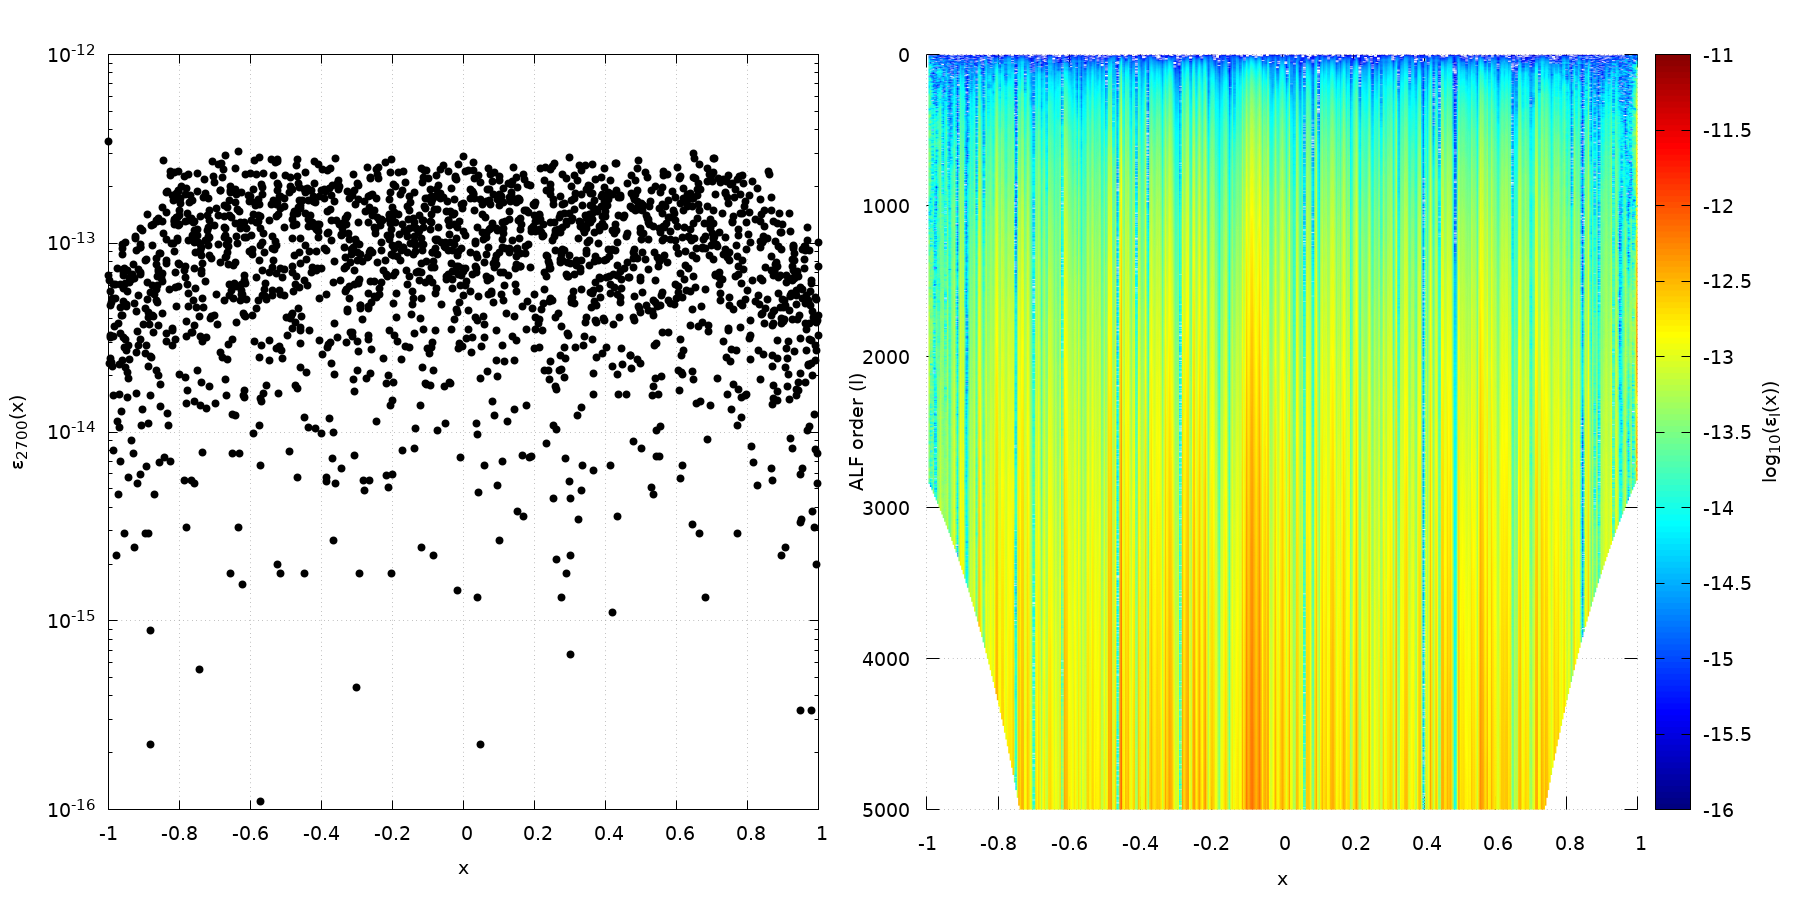
\includegraphics[width=\textwidth]{plots/legeps.png}
\caption{Left: $\epsilon_{2700}(x)$ for $2000$ randomly distributed points
on $[-1,1]$. Right: Map of $\log_{10}(\epsilon_l(x))$ as a function of
ALF degree $l$ and $x$. Schmidt normalization is used.
}
\label{fig:legeps}
\end{figure}

A useful method for testing the accuracy of high degree and order
ALFs is to use the following identity for the Schmidt quasi-normalized
ALFs,
\begin{equation}
\sum_{m=0}^l \left( S_l^m(x) \right)^2 = 1 \label{eqn:S1}
\end{equation}
We define the following quantity for testing purposes,
\begin{equation}
\epsilon_l(x) = \sum_{m=0}^l \left( S_l^m(x) \right)^2 - 1
\end{equation}

Figure~\ref{fig:legeps} (left) shows the value of $\epsilon_{2700}(x)$
for 2000 randomly chosen points $x$ on $[-1,1]$. The right panel shows
a heat map of $\log_{10}(\epsilon_l(x))$ as a function of degree $l$ and
input $x$.

\subsection{Comparison with arbitrary precision libraries}

\begin{figure}[ht]
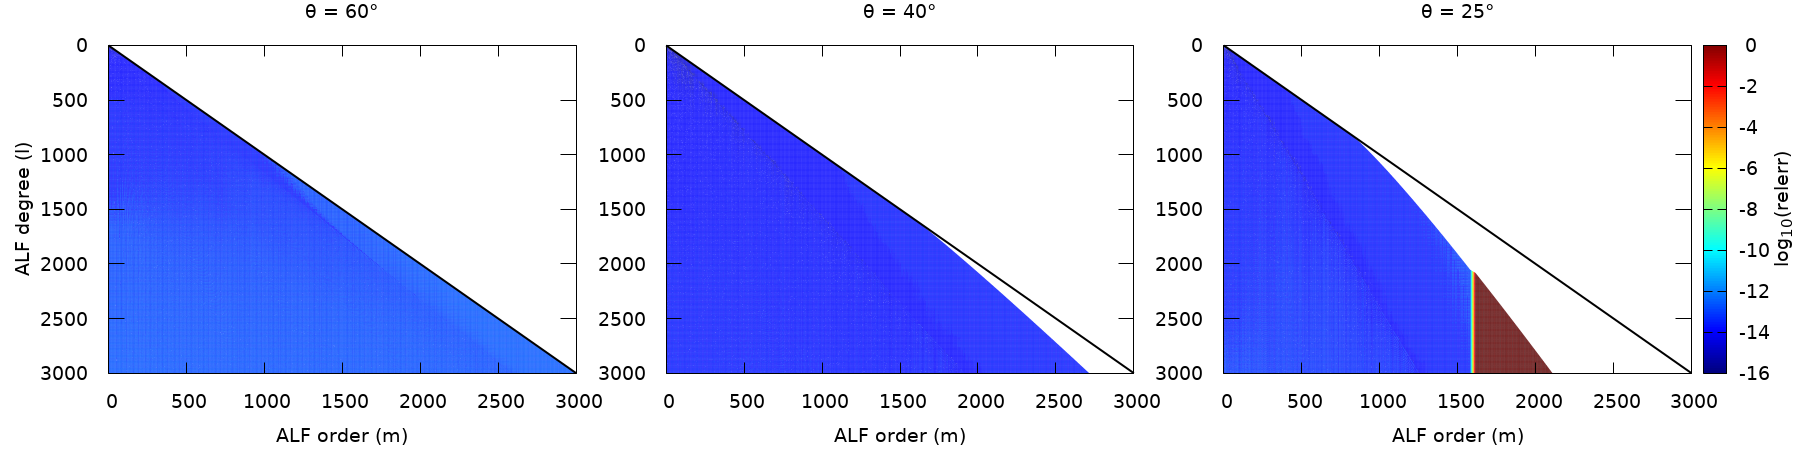
\includegraphics[width=\textwidth]{plots/compare.png}
\caption{
Log of relative error between GSL and mpmath calculations plotted versus
ALF degree and order for $\theta = 60^{\circ}$ (left),
$\theta = 40^{\circ}$ (middle),
$\theta = 25^{\circ}$ (right). This figure uses the spherical
harmonic normalization.
}
\label{fig:compare}
\end{figure}

Here, we compare the GSL ALF calculation against the
arbitrary precision Python library, mpmath, using a working
precision of 50 digits. In the case of ALFs, arbitrary precision
libraries avoid the underflow problem at high orders, and can
serve as a truth reference for the double precision GSL calculations.
Figure~\ref{fig:compare} presents the logarithm of the relative error
between GSL and mpmath, using spherical harmonic normalized ALFs up to
degree and order 3000, for three different input values, $x = \cos{\theta}$.
The left panel shows $\theta = 60^{\circ}$, the middle panel
$\theta = 40^{\circ}$, and the right panel $\theta = 25^{\circ}$. The
whitespace under the black diagonal line indicates that the resulting
ALF cannot be represented in double precision, and the GSL calculation
underflowed. We see that the underflow problem increases as we move
closer to the pole region at high degrees and orders. The blue regions
indicate that GSL matches the arbitrary precision result to around 12-16
significant digits. The red portion of the right panel indicates a
loss of many significant digits in the GSL result, starting around
degree 2000 and order 1500 for $\theta = 25^{\circ}$.

\section{Benchmarks}

\begin{figure}[ht]
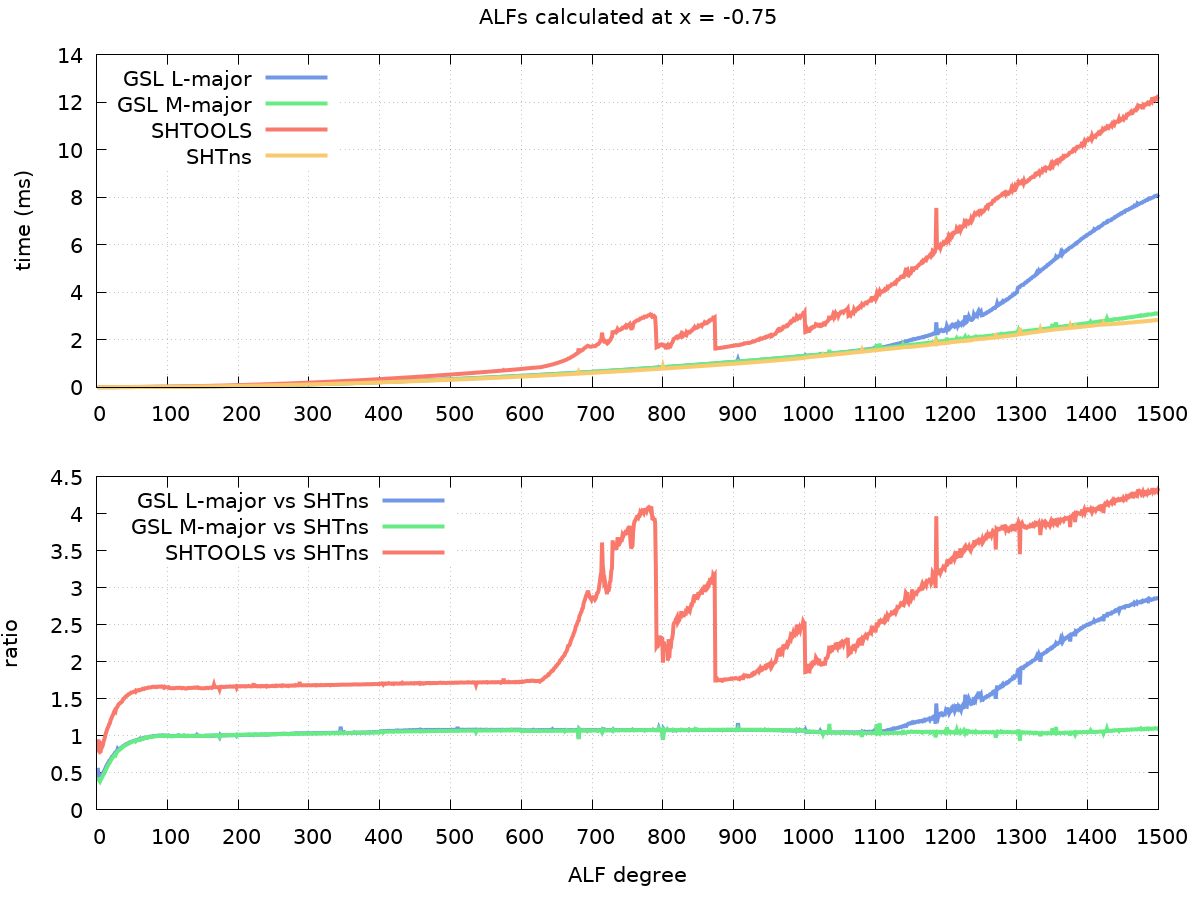
\includegraphics[width=\textwidth]{plots/bench.png}
\caption{Top: Average time of ALF calculation for different libraries as a function of ALF
degree, for the input $x = -0.75$. Bottom: Ratio of library times to the SHTns library.}
\label{fig:bench}
\end{figure}

Here, we compare the performance of the GSL implementation of ALFs
against two other libraries. The first, known as SHTOOLS
\citep{wieczorek2018}, provides numerous normalization conventions
and uses L-major indexing in the output arrays. The second,
called SHTns \citep{schaeffer2013}, provides highly optimized ALFs
with the spherical harmonic normalization, and uses M-major indexing
in its output arrays. All benchmarks were performed on an Intel Xeon
CPU E5-2620 v3 @ 2.40GHz with 64GB RAM. Figure~\ref{fig:bench} presents the result of
calculating ALFs using each library interface for a fixed input point
$x = -0.75$. The top panel displays the wall clock time for each
implementation as a function of ALF degree up to $L = 1500$. The
SHTns and GSL implementions (with M-major indexing) perform best at
nearly all degrees, with SHTns performing slightly faster than GSL.
The bottom panel shows the wall clock time compared with SHTns (e.g.
the ratio between the GSL/SHTOOLS time and SHTns). The green
curve shows that GSL (M-major indexing) performs nearly as well as SHTns
at all degrees up to 1500. The blue curve shows that GSL (L-major indexing)
is competitive with SHTns up to about degree 1100 at which point it
begins to significantly underperform. The SHTOOLS library underperforms
SHTns at all degrees, which we attribute to its cache-inefficient implementation.
The source code used for these benchmarks is listed in Appendix~\ref{sec:benchsrc}.

\section{List of Acronyms}

\begin{tabular}{@{}ll@{}}
\toprule
Acronym & Meaning \\
\midrule
ALF & Associated Legendre Function \\
GSL & GNU Scientific Library \\
\bottomrule
\end{tabular}

\bibliographystyle{unsrtnat}
\begin{thebibliography}{10}

\bibitem[Bosch, 2000]{bosch2000} Bosch, W., ``On the computation of derivatives of Legendre functions,'', \emph{Phys. Chem. Earth}, 25, 9--11, pg. 655--659, 2000.

\bibitem[Galassi et al, 2009]{GSL} Galassi, M., Davies, J., Theiler, J., Gough, B., Jungman, G., Alken, P., Booth, M., and Rossi, F., ``GNU Scientific Library Reference Manual,'' 3rd edition, \emph{Network Theory Ltd}, 2009.

\bibitem[Holmes and Featherstone, 2002]{holmes2002} Holmes, S., Featherstone, W., ``A unified approach to the Clenshaw summation and the recursive computation of very high degree and order normalised associated Legendre functions,'' \emph{Journal of Geodesy}, 279-299, 2002.

\bibitem[Schaeffer, 2013]{schaeffer2013} Schaeffer, N., ``Efficient spherical harmonic transforms aimed at pseudospectral numerical simulations'', \emph{Geochem. Geophys. Geosys.}, 14, 3, 751--758, doi:10.1002/ggge.20071, 2013.

\bibitem[Wieczorek and Meschede, 2018]{wieczorek2018} Wieczorek, M. A., Meschede M., ``Tools for working with spherical harmonics'', \emph{Geochem. Geophys. Geosys.}, 19, 2574--2592, doi:10.1029/2018GC007529, 2018.

\bibitem[Winch, 2005]{winch2005} Winch, D. E., Ivers, D. J., Turner, J. P. R., and Stening, R. J., ``Geomagnetism and Schmidt quasi-normalization,'' \emph{Geophys. J. Int.}, 160, p. 487-504, 2005.

\end{thebibliography}

\appendix

\section{Source Code for Benchmarks}
\label{sec:benchsrc}

The following code was used to generate Figure~\ref{fig:bench}. It was compiled with the
command:
\scriptsize
\begin{verbatim}
g++ -O2 -Wall -W -o bench bench.cc -lm -lgsl -lshtns -lfftw3 -lSHTOOLS -llapack -lcblas -lf77blas -lgfortran
\end{verbatim}

\lstinputlisting[language=c++]{src/bench.c}

\end{document}
